%Conditions for paper extension:

%1. The extended version must have at least 30% of novel contents. This can include new experiments, demonstrations, more datasets, comparisons with the literature, proofs of theorems, and so on. Some few paragraphs of insignificant text is absolutely not sufficient.
%2. The authors should enrich the paper structure, by avoiding to maintain exactly the same sequence and numbering of sections.
%3. The title must be different from that of the paper published in the conference proceedings.
%4. Please strictly avoid verbatim repetitions, i.e., large blocks of text copied from the conference paper (for example, abstract, introduction and conclusions) as they are: this can be considered as self-plagiarism.
%5. Properly cite the paper published in the conference proceedings, and clearly describe in the introduction the differences between the two papers.
%6. If you use any table, figure or equation that was used in the conference paper then you need to refer where it was published, for example including a citation in the caption.

\documentclass[runningheads]{llncs}

\usepackage[T1]{fontenc}
\usepackage{graphicx}
\usepackage{hyperref}
\usepackage{caption}
\usepackage{subcaption}
\usepackage{wrapfig}
\usepackage[linewidth=1pt]{mdframed}
%\usepackage{color}
%\renewcommand\UrlFont{\color{blue}\rmfamily}

\begin{document}

\title{Exploring Semantic Similarity between German Legal Texts and Referred Laws}
%\titlerunning{Abbreviated paper title}

\author{Harshil Darji\orcidID{0000-0002-8055-1376} \and
Jelena Mitrović\orcidID{0000-0003-3220-8749} \and
Michael Granitzer\orcidID{0000-0003-3566-5507}}

\authorrunning{Darji et al.}

\institute{Chair of Data Science, University of Passau, Innstraße 41, 94032 Passau, Germany
\email{\{harshil.darji, jelena.mitrovic, michael.granitzer\}@uni-passau.de}}

\maketitle

\begin{abstract}
The calculation of semantic similarity is an important task in Natural Language Processing (NLP). There is a growing interest in this task in the research community, especially following the advent of new, ever-evolving neural architectures. However, this technique has not been explored in-depth in the realm of automatic processing of legal data, the area we often call Legal NLP or Legal Tech. In this paper, we aim to use semantic similarity to identify the relations between legal sentences that refer to a certain law and the law text itself. The semantic similarity score is calculated using cosine similarity between sentence embeddings. In our work, we use sentence transformers to get the sentence embeddings for our legal text. The results we achieve by using two separate sentence transformers, Cross English \& German RoBERTa and all-MiniLM-L6-v2, provide a semantic similarity score of approximately 0.45 and 0.4, respectively.

% The comparison of legal sentences that refer to the same base law also suggests that they are closely grouped in embedding space. Our work shows that there do exist semantic similarities between the legal text and the law text. This score can be improved by using new or improved embedding techniques, which can further assist in predicting law references, identifying similar court cases and court decisions, and legal text entailment.

\keywords{Legal Language Processing \and NLP \and Semantic Similarity \and Sentence Transformers \and Open Legal Data.}
\end{abstract}

% -------------------------------------------------------
% -------------------- INTRODUCTION ---------------------
% -------------------------------------------------------

\section{Introduction}
\label{sec:introduction}

Investments in global legal technologies, supporting various stages of legal processes and proceedings, have grown from 17.32 billion U.S. dollars in 2019\footnote{\url{https://www.statista.com/statistics/1155852/legal-tech-market-revenue-worldwide/}} to 18.4 billion U.S. dollars in 2021\footnote{\url{https://www.statista.com/topics/9197/legal-tech/}}. The legal research community has also taken note of this growing interest and is working toward applying the latest AI and Machine Learning technologies to build tools that can assist in efficient legal research. Research in legal tech differs based on the underlying legal system and countries. NLP-based systems adjust accordingly to investigate which studies can be translated and replicated across these different manifestations of the legal domain.

There exist different NLP tools and techniques, some are rule-based that focus more on pattern matching or fill-in-the-blanks tasks. Such methods, although proven to work well, do not work efficiently when generalized. Other tools are based on Machine Learning models, where some use probabilistic or linear classifiers while others use a state-of-the-art neural networks. However, the introduction of Transformers\cite{vaswani2017attention} in 2017 gave rise to improved and more efficient NLP tools such as BERT\cite{devlin2018bert}, RoBERTa\cite{liu2019roberta}, etc.

With an increasing amount of new cases, improved NLP tools are effective to gather important legal information, which is necessary to generate citation networks for legal purposes. Such citation networks can reveal critical information on precedents \cite{Cross2010CITATIONSSIGNIFICANCE} based on the characteristics of the citations towards the precedent candidates. In previous work by Milz et al. \cite{milz2021analysis}, the authors demonstrated the scale-free behavior of the German case citation network. This citation network was built using a dataset similar to the one we use in our current work. They also make use of the PageRank algorithm to identify the most influential court decisions and laws. And finally, they claim the positive correlation between node- and text-based similarity scores. The citation network developed in their work is helpful for understanding court decisions, finding similar court cases based on similar court decisions, and finding background knowledge for a given case. However, for this to work, it requires manual reference to norms, which is not always feasible. For retrieval systems that do not rely on such manual annotations, it is necessary to utilize textual similarity techniques. In addition, we might also be able to conduct further analysis and downstream tasks such as developing a system that can differentiate between tenor and gründe using semantic similarities and also identifying clustering reasons in court decisions.

Our work is an extension of the original paper by Milz et al.\cite{milz2021analysis} titled "\textit{Analysis of a German Legal Citation Network}". In this work, instead of using law references to identify node similarities, we try to identify similarities between the law text and legal text that refer to a given law. Additionally, legal sentences that refer to the same law should likely be semantically similar as well. To show this, we also work on finding semantic similarities between legal sentences that refer to the same law. The results from our experiment confirm that semantic similarity can be exploited to reference similar law texts. Semantic similarity between sentences or documents plays a significant role in Automated Short-Answer Grading, Machine Translation, and Image Captioning\cite{sanborn2015deep}. Techniques such as TF-IDF and Bag-of-Words (BoW) represent text as real-value vectors that can be used to find semantic similarity, but they do not account for the fact that similar words sometimes can have a different meaning or different words can sometimes be used to represent similar concepts \cite{chandrasekaran2021evolution}.

Here, we use sentence transformers to generate sentence embeddings. A sentence transformer is a modification of the pre-trained BERT network that uses siamese and triplet network structures to derive semantically meaningful sentence embeddings\cite{reimers2019sentence}. These embeddings can then be compared using cosine-similarity to get a semantic similarity score. We use Cross English \& German RoBERTa for Sentence Embeddings from T-Systems-onsite\footnote{\url{https://huggingface.co/T-Systems-onsite/cross-en-de-roberta-sentence-transformer}} and all-MiniLM-L6-v2\footnote{\url{https://huggingface.co/sentence-transformers/all-MiniLM-L6-v2}} to generate embeddings and compare the performance of both.

Our paper is structured as follows: In section \ref{sec:related_work}, we summarise some of the related work in this field and indicate how our work can provide new insights into this area of research. In section \ref{sec:dataset}, we give details about the used dataset and how it differs from the original work. Next, in section \ref{sec:law_net}, we briefly summarise the work done by Milz et al. in the original work. In section \ref{sec:experiment}, we give details about the experiments done before presenting the results in \ref{sec:results}.

% -------------------------------------------------------
% -------------------- RELATED WORK ---------------------
% -------------------------------------------------------

\section{Related Work}
\label{sec:related_work}

In 2006, Li et al.\cite{li2006sentence} presented an algorithm that makes use of semantic and word order information. Because their algorithm derives semantic similarity from a lexical knowledge base and a corpus, it can adapt to different application areas using a corpus of that area. They evaluated their similarity algorithm on a set of sentence pairs from a variety of sources and achieved performance comparable to human participants.

In 2014, Kim et al.\cite{kim2014legal} published their work on legal Q\&A using Ranking SVM and syntactic or semantic similarity. The dataset used by the authors for the evaluation is the first competition on legal information extraction/entailment (COLIEE) 2014, with two phases. The first phase was the identification of the relevance of Japanese civil law articles to a legal bar exam query. For this, they compared two baseline unsupervised models with Ranking SVM and concluded that the latter achieved performance far better than baseline models. In the second phase, they answer "yes" and "no" questions by comparing the query's meanings with the corresponding articles. For this purpose, they use semantic similarities with antonym relation identification. The authors claim that their method, combined with the rule-based model and the unsupervised model, outperforms the SVM-based supervised model. 

In 2016, Mueller et al.\cite{Mueller_Thyagarajan_2016} presented a siamese adaptation of the LSTM network to calculate semantic similarity between sentences. Their approach benefits from improved word-embeddings of sentences as pre-trained word-vectors are used as LSTM input. Furthermore, they form a highly structured space with complex semantic relationships by relying on a simple Manhattan metric\cite{garner1963iterative}. Their results conclude that LSTMs are capable of effectively performing tasks that require complex understanding.

In 2020, Zhong et al.\cite{zhong2020does} published a paper explaining the use of NLP in legal tech. In addition, they also provide advantages and disadvantages of existing methods. Their work provides a comprehensive overview of different embedding-based and symbol-based methods. They conclude that although existing methods can provide good results for element extraction, they are not sufficient for corresponding applications. 

In 2020, Paheli et al.\cite{bhattacharya2020methods} published their work on computing similarity between two legal documents. In this, they explored text-based and network embeddings-based methods for similarity computation on a set of 47 document pairs. Based on the Pearson correlation between the expert score and similarity implied by methods used, Node2Vec performed best for citation network-based measures while FullText Similarity achieved good performance for text-based measures.

Milz et al. published their work on German legal citation networks\cite{milz2021analysis}. In this, they used the Jaccard similarity score between all pairs of nodes to identify similar court decisions. They compared the results of node similarity with simplified text-based similarity calculation. The results show that both similarity scores are in agreement more often. Furthermore, they performed a Pearson correlation test between the similarity measures of 1000 semi-randomly chosen court decisions and achieved a score of 0.64, implying a positive correlation.

In addition, another important research in terms of the use of NLP in German legal data was done by Leitner et al.\cite{leitner2019fine} in 2019. Here, they created a dataset of Named Entity Recognition with 19 fine-grained classes, that can be generalized into seven coarse-grained classes. Then, they applied Conditional Random Fields (CRFs) and bidirectional Long-Short Term Memory Networks (BiLSTMs) to this NER dataset. Out of these two state-of-the-art models, BiLSTMs have better performance with an F1 score of 95.46 for the fine-grained and 95.95 for the coarse-grained classes.

To the best of our knowledge, there is no work on using sentence transformers to calculate semantic similarities between German legal texts. On the other hand, some research on using transformers for sentence similarity modeling does exist . For example, Laskar et al.\cite{laskar2020contextualized} used contextualized word embeddings with the transformer encoder for the answer selection task. In this work, the authors presented feature-based and fine-tuning-based approaches for answer selection. In another work, Ormerod et al.\cite{ormerod2021predicting} utilized independently fine-tuned transformers to calculate the average predicted similarity score.

% -------------------------------------------------------
% ----------------------- DATASET -----------------------
% -------------------------------------------------------

\section{Dataset}
\label{sec:dataset}

There is a noticeable discrepancy between the legal tech research output in North American and Europe.This is largely due to the lack of publicly available data in Europe. For example, there is a public dataset of 3.7 million U.S. precedential court decisions. Furthermore, Google search engine provides the option of searching through a vast data collection of the U.S. Case law. In European countries, Germany in particular, apart from the commercial datasets, there are only around 55000 publicly available court cases from the State Ministry of Justice (ger. Bundesministerium der Justiz). Many states in Germany also publish some records individually but do not allow users to scrape their content. This makes it difficult to have a centralized and openly available source for German legal data.

Ostendorff et al.\cite{ostendorff2020towards} recognized this and published an openly available dataset called Open Legal Data. This dataset was used by Milz et al. in the original paper\cite{milz2021analysis} to create a German citation network for legal data. The first step toward creating such a citation network is to extract citations from the decision text of cases. Due to the lack of distinctly identifiable references to previous court decisions or laws, extracting citations was not an easy task.

One of the reasons for this complication in extracting case-to-case citations is the lack of a properly structured unique identifier for court decisions. European Case Law Identifier can solve this problem, but this was only introduced in 2011, and not all the cases use it. In regards to law reference extraction, Milz et al. only considered citations that begin with the article sign ("§"). If there are multiple law references, they avoided such inconsistency by using the double article sign ("§§"). Overall they managed to extract 1,279,105 case-to-case citations and 2,234,934 case-to-law citations.

We tackle this problem of extracting the information from Open Legal Data in a different way. This dataset clearly mentioned information such as court, level of appeal, and ECLI. However, important text such as tenor, tatbestand, gründe, and entscheidungsgründe was available only in HTML format. One of the complications in extracting information from HTML was the inconsistency of HTML structure throughout the dataset. For example, not all the cases in the dataset use the same tags or identifiers to separate title from content.

Due to these inconsistencies in HTML structure in the dataset, we had to make some assumptions to extract the information from them. One of which was to assume that all the important titles, such as tenor and gründe are within the \textit{h2} tag. In addition, to avoid false positives, we also made sure the content within \textit{h2} tag is all alphabetic and is within a certain length. These assumptions lowered the number of cases to 43337.

The size of the resulting dataset is approximately ~1.1 GBs, with 43337 rows and has the following 12 features:
\begin{table}[!h]
	\centering
	\begin{tabular}{|c|c|l|}
	    \hline
		\textbf{Feature} & \textbf{Total} & \textbf{Example content}\\
		\hline
		id & 43337 & 127981\\
		slug & 43337 & ag-volklingen-2002-07-10-5c-c-24102\\
		ecli & 10831 & NaN\\
		date & 43337 & 2002-07-10\\
		court & 43337 & Amtsgericht Völklingen\\
		jurisdiction & 43337 & Ordentliche Gerichtsbarkeit\\
		level\_of\_appeal & 43337 & Amtsgericht\\
		type & 43337 & Urteil\\
		tenor & 36282 & 1. Die Beklagten werden als Gesamtschuldner...\\
		tatbestand & 24243 & Auf die Darstellung des Tatbestandes...\\
		gründe & 27144 & Die Klage ist zulässig und begründet. Die...\\
		entscheidungsgründe & 24038 &  Die Klage ist zulässig und begründet. Di...\\
		\hline
	\end{tabular}
	\caption{Features in the dataset with statistics and example content. Here, \textit{slug} can be used to view the web-version of any case by appending it to \textit{https://de.openlegaldata.io/case/<slug>}.}
	\label{tab:data_example}
\end{table}

One of the important features in this dataset is ECLI, an abbreviation for European Case Law Identifier. This identifier consists of five elements, separated by colons, \textbf{ECLI:[the country code]:[the code of the court]:[the year]:[an ordinal number]}\footnote{\url{https://e-justice.europa.eu/content_european_case_law_identifier_ecli-175-en.do}}.

The plot in figure \ref{fig:case_per_year} shows the number of cases per year, from 2002 to 2019. The reason for having very few cases in 2019 compared to previous years is because the data obtained from Open Legal Data only included cases up to the year 2019.

\begin{figure}[!h]
	\centering
	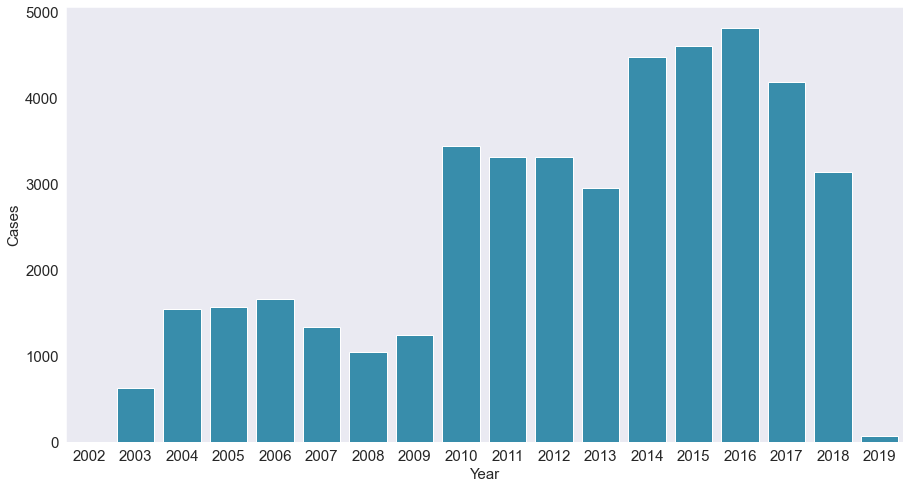
\includegraphics[width=0.63\linewidth]{images/year_case.png}
	\caption{Number of cases per year, 3 cases in 2002 and highest being in 2016.}
	\label{fig:case_per_year}
\end{figure}

This dataset is publicly available and can be downloaded from the provided link\footnote{\url{https://zenodo.org/record/6631931\#.YqNkbxNBz0o}}.

% -------------------------------------------------------
% --------------------- DE LAW NET ----------------------
% -------------------------------------------------------

\section{German law citation network}
\label{sec:law_net}

\begin{figure}
    \centering
    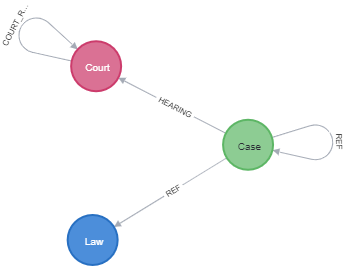
\includegraphics[width=0.5\linewidth]{images/node.png}
   \caption{Neo4j graph of the legal citation network\cite{milz2021analysis}.}
   \label{fig:graph_simple}
\end{figure}

Milz et al. \cite{milz2021analysis} constructed a legal citation network for the German legal data. As stated in their work, they present a case-to-case citation network that also connects cases to the laws that are referenced within their decision text, as shown in figure \ref{fig:graph_simple}. Table \ref{tab:properties} shows the properties of nodes in the legal citation graph. Exactly one directed edge exists between two Case nodes (n) and (m) if (n) references (m) in the decision text at least once. For their analysis, it is of importance that a reference occurs, but not how often. Hence, multiple references from the same decision text to the same node are disregarded.

\begin{table}[h]
\centering
\vspace{0.2cm}
\begin{tabular}{|c|c|p{3.5cm}|}

  \hline
   \textbf{Node}&\textbf{Property} &  \textbf{Example} \\
  \hline
Case & DecisionText & Der Antrag des Antragstellers, § 1 Abs. 5 Corona VV HE 4 im Wege der einstweiligen Anordnung...\\
  \hline
   Case&File Number & IX ZR 70/20\\
  \hline
   Case&Decision Date & 25.03.2021\\
  \hline\hline
  Law&Article & § 242\\
    \hline
  Law&Statute & BGB\\
  \hline
  Law&Law Text & Der Schuldner ist verpflichtet, die Leistung so zu bewirken...\\
  \hline\hline
  Court&Name & Finanzgericht Hamburg\\
  \hline
  Court&State & Hamburg\\
  \hline
  Court&Jurisdiction & Finanzgerichtsbarkeit\\
  \hline
\end{tabular}
\caption{Node properties of the legal citation graph\cite{milz2021analysis}}\label{tab:properties}
\end{table}

The authors here ignored the laws or court decisions that are not yet in the dataset since an edge cannot be added between nodes that do not exist in the dataset. Because of this, only 59.9\% of law references can be added as edges, while only 16.3\% of court decision references are represented in the graph.

\subsection{Scale-free Network}

Similar to the case citation networks of the U.S. Supreme Court \cite{Smith2005TheLaw}, the Austrian Supreme Court \cite{Geist2009UsingJurisdictions} and the European Court of Justice \cite{StaffanMalmgren2011TowardsLaw}, German legal citation network also shows scale-free behavior. This behavior reveals that a very small cluster of court decisions holds a substantial amount of legal influence. This conclusion has been made considering the fact that the citation network shows that more than 70\% of court decisions are not cited at all, and 92.6\% of cases are cited less than five times.

This scale-free behavior is confirmed based on the case-to-case in-degree and case-to-law in-degree diagram (figure \ref{fig:in-degree}). As stated by the authors, "case and law references are not equally distributed, but there are in fact hub-like decisions and laws that are more likely to be cited".

\begin{figure}[!h]
     \centering
     \begin{subfigure}[b]{0.49\textwidth}
         \centering
         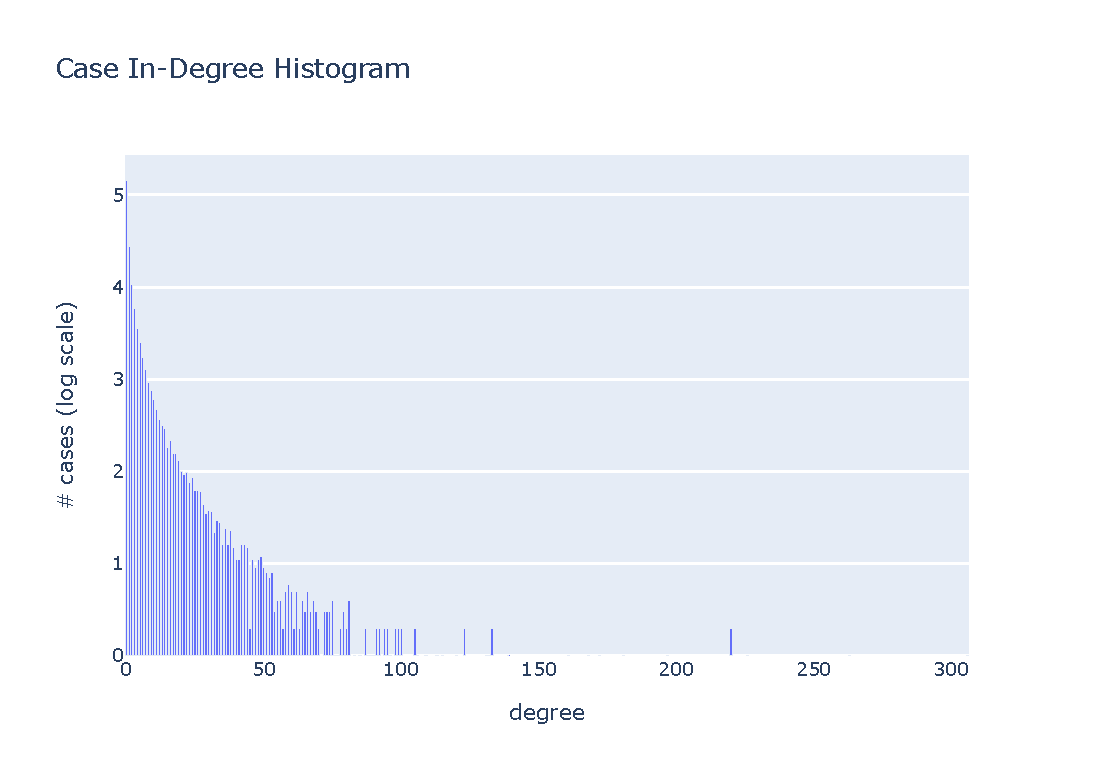
\includegraphics[width=\textwidth]{images/indegree_case.pdf}
         \caption{Case-to-Case In-Degree distribution}
     \end{subfigure}
     \hfill
     \begin{subfigure}[b]{0.49\textwidth}
         \centering
         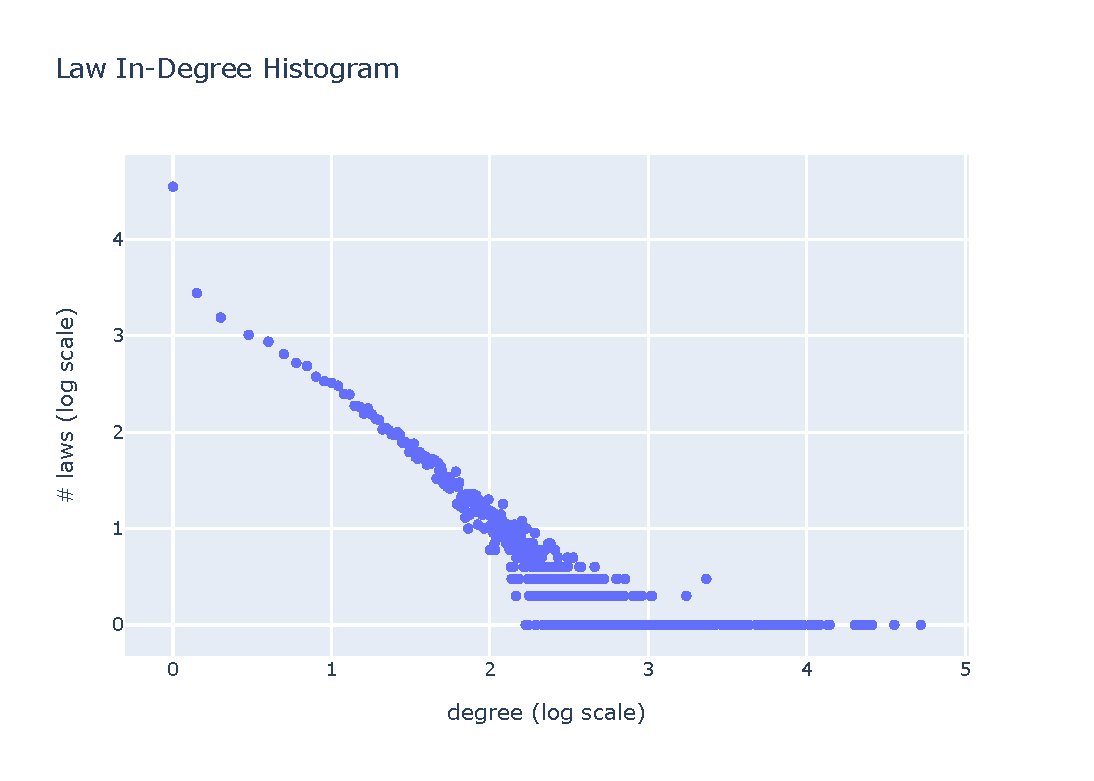
\includegraphics[width=\textwidth]{images/indegree_law.pdf}
         \caption{Case-to-Law In-Degree distribution}
     \end{subfigure}
    \caption{Case and Law In-Degree distribution with log scale. This type of distribution suggests a scale-free network behaviour \cite{milz2021analysis}.}
    \label{fig:in-degree}
\end{figure}

\subsection{Centrality}

One of the major aspects of legal research is to identify the most influential and important court decisions and precedents. One of the common practices to measure excellence is to count citations. In Milz et al. work, In-degree and PageRank scores have shown to be strong indicators for identifying precedents and influential cases. Figure \ref{fig:top_20_pr} shows the twenty most important court decisions based on their overall PageRank rating. Figure \ref{fig:pr_1o_year} shows the top three decisions based on PageRank, but with respect to the year of the case.

\begin{figure}[!h]
     \centering
     \begin{subfigure}[b]{0.49\textwidth}
         \centering
         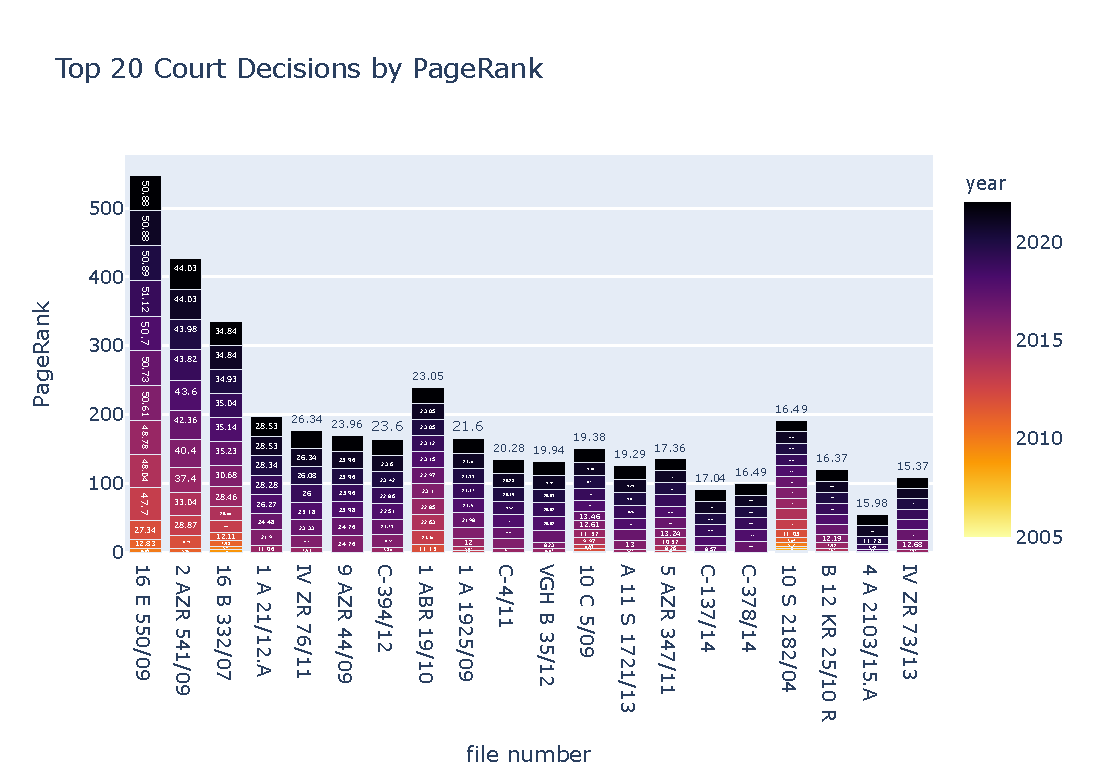
\includegraphics[width=\textwidth]{images/top20ByPagerank.pdf}
         \caption{This stacked bar shows the most influential court decisions based on their PageRank score. As depicted in the chart, most decisions become highly influential after the third year of their appearance.}
         \label{fig:top_20_pr}
     \end{subfigure}
     \hfill
     \begin{subfigure}[b]{0.49\textwidth}
         \centering
         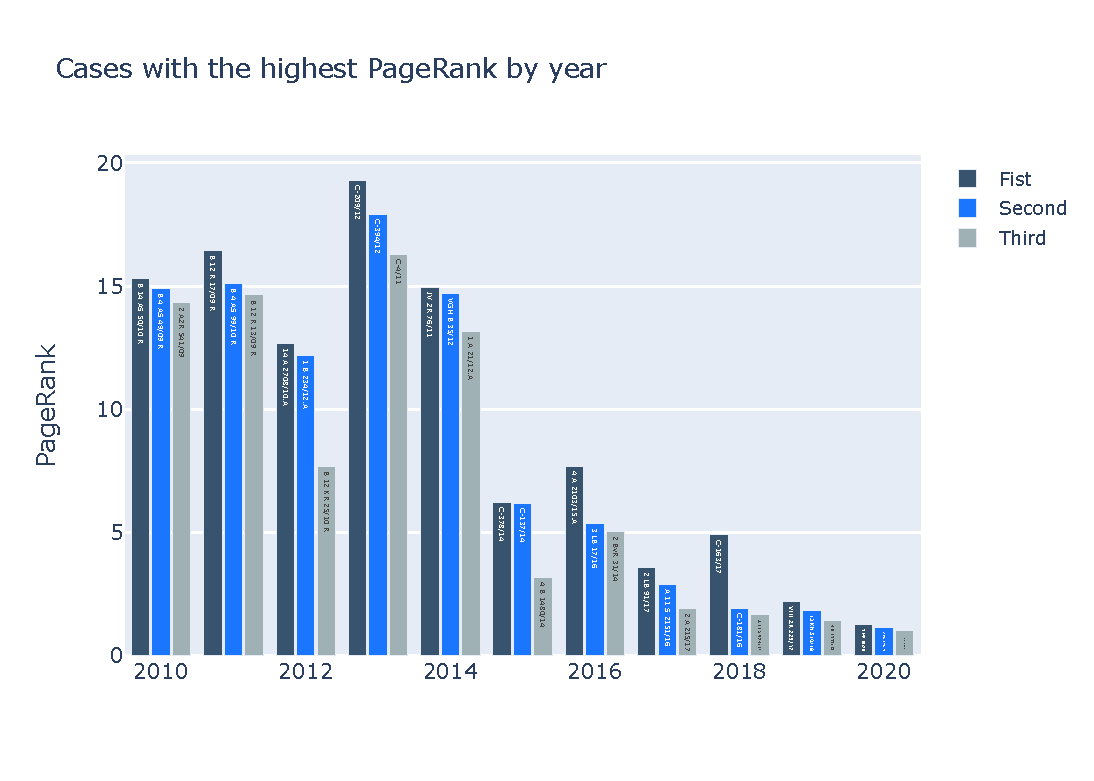
\includegraphics[width=\textwidth]{images/PageRankLast10Years.pdf}
         \caption{This plot shows the top three court decisions based on PageRank by year. This visualization shows that in some years the most important decisions were made by the European Court of Justice.}
         \label{fig:pr_1o_year}
     \end{subfigure}
    \caption{Top-20 most influential court decisions and top-3 decisions based on their respective PageRank score \cite{milz2021analysis}.}
\end{figure}

\subsection{Node similarity}

An important task of legal research is the identification or discovery of similar cases based on court decisions, topics, or law references. Previous work in this area has shown that despite being perspective to sparsity, network-based similarity does work. Milz et al. \cite{milz2021analysis} used the Jaccard algorithm to find similarities between court decisions by calculating node similarity scores between all pairs of nodes in the Neo4j graph. The Jaccard algorithm considers a pair of nodes as similar if they share the majority of neighbors. Then as mentioned in section \ref{sec:related_work}, they compared this score with a text-based similarity measure to find a correlation.

\begin{table*}[h!]
\centering
\begin{tabular}{|l|l|c|c|}
\hline
      Case1 &        Case2 &  Node Similarity &  TF-IDF Similarity \\\hline
\hline
 VI-3 Kart 18/09 (V) &  VI-3 Kart 17/09 (V) &             1.00 &               1.00 \\\hline
 VI-3 Kart 18/09 (V) &  VI-3 Kart 26/09 (V) &             1.00 &               1.00 \\\hline
 VI-3 Kart 18/09 (V) &  VI-3 Kart 27/09 (V) &             1.00 &               0.99 \\\hline
 VI-3 Kart 18/09 (V) &  VI-3 Kart 28/09 (V) &             1.00 &               0.99 \\\hline
 VI-3 Kart 18/09 (V) &  VI-3 Kart 29/09 (V) &             1.00 &               0.99 \\\hline\hline
 W 7 M 19.30082 &  W 7 M 19.30083 &             1.00 &               0.96 \\\hline
 W 7 M 19.30082 &  5 L 1635/14.TR &             0.88 &               0.69 \\\hline
 W 7 M 19.30082 &  17 L 1610/14.A &             0.81 &               0.71 \\\hline
 W 7 M 19.30082 &   7 L 1224/14.A &             0.58 &               0.55 \\\hline
 W 7 M 19.30082 &      3 E 187/17 &             0.50 &               0.53 \\\hline\hline
  L 8 R 208/05 &  L 8 R 361/06 &             1.00 &               0.98 \\\hline
 L 8 R 208/05 &   L 8 R 44/06 &             0.86 &               0.97 \\\hline
 L 8 R 208/05 &   L 8 R 47/06 &             0.86 &               0.13 \\\hline
 L 8 R 208/05 &   L 8 R 62/07 &             0.80 &               0.97 \\\hline
 L 8 R 208/05 &   L 3 R 98/05 &             0.35 &               0.97 \\\hline
\hline
\end{tabular}
\caption{Comparison between node similarity and TF-IDF based text-similarity \cite{milz2021analysis}.}
\label{tab:similarityTable1}
\end{table*}

Some examples of this comparison are shown in table \ref{tab:similarityTable1}. As indicated by the scores in this table, node-based and text-based similarity scores agree more often. This agreement is quantified by calculating the Pearson correlation between the similarity measures of 1000 semi-randomly chosen court decisions and five corresponding counterparts. The positive correlation score of 0.64 indicates that case-similarity search methods can be further improved by adding network-based similarity measures.

% -------------------------------------------------------
% -------------------- EXPERIMENTS ----------------------
% -------------------------------------------------------

\section{Experiments}
\label{sec:experiment}

Our experiments in this publication focus on extending the similarity measures from node-similarity to textual or semantic similarities. Here, we focus on sentence-level text information instead of comparing entire cases. We use law references to not only compare their text with legal sentences that refer to them but also to compare legal sentences that refer to the same sentence.

\subsection{Similarity between law text and legal sentences}

In the first experiment, we aim to find semantic similarities between the sentences from a legal case that refer to a law and the actual text from that law. To do so, one of the tasks here is to extract the law reference from the case. We extracted the law references directly from the HTML file. Most of the law references in the original Open Legal Data are within \textit{verweis.norm} tag. We simply extracted the content within this tag and replaced the "Art." or "§§" sign with "§". Next, we gather the legal text from cases that surrounds these law references.

Since no API for getting a specific law and Absatz text exists, we relied on extracting this information from \textit{Gesetze im Internet, Bundesministerium der Justiz}\footnote{\url{https://www.gesetze-im-internet.de/}}. Because of a consistent HTML structure, we we were able to extract both the entire law text and the Absatz text. 

After having the legal sentence and law text, the next step is to gather embeddings for both. This is done by feeding both the sentences to two separate sentence transformers, namely Cross English \& German RoBERTa for Sentence Embeddings and all-MiniLML6-v2. One of the reasons for choosing sentence transformers above traditional techniques such as TF-IDF is their ability to account for the fact that similar words can have different meanings based on context and vice versa.

Finally, we calculate the cosine similarity between these two embeddings to get the semantic similarity between the legal sentence and the corresponding law text.

The process of finding this semantic similarity is explained below with an example. Consider the following legal sentence:\\

\begin{mdframed}
\textit{... Leben oder Freiheit besteht. Eine erhebliche konkrete Gefahr aus gesundheitlichen Gründen liegt nur vor bei lebensbedrohlichen oder schwerwiegenden Erkrankungen, die sich durch die Abschiebung wesentlich verschlechtern würden (§ 60 Abs. 7 Satz 2 AufenthG). Es ist ...}
\end{mdframed}

In this text, we can see one of the law's references is \textit{§ 60 Abs. 7 Satz 2 AufenthG}. We extract the law text of this law from \textit{Gesetze im Internet}\footnote{\url{https://www.gesetze-im-internet.de/aufenthg_2004/__60.html}}, which says:

\begin{mdframed}
\textit{... Es ist nicht erforderlich, dass die medizinische Versorgung im Zielstaat mit der Versorgung in der Bundesrepublik Deutschland gleichwertig ist. ...}
\end{mdframed}

We then simply get the embeddings of both texts using sentence transformers and find the cosine similarity between both embeddings. The following chart shows the simplified process of this experiment:

\begin{figure}[h]
	\centering
	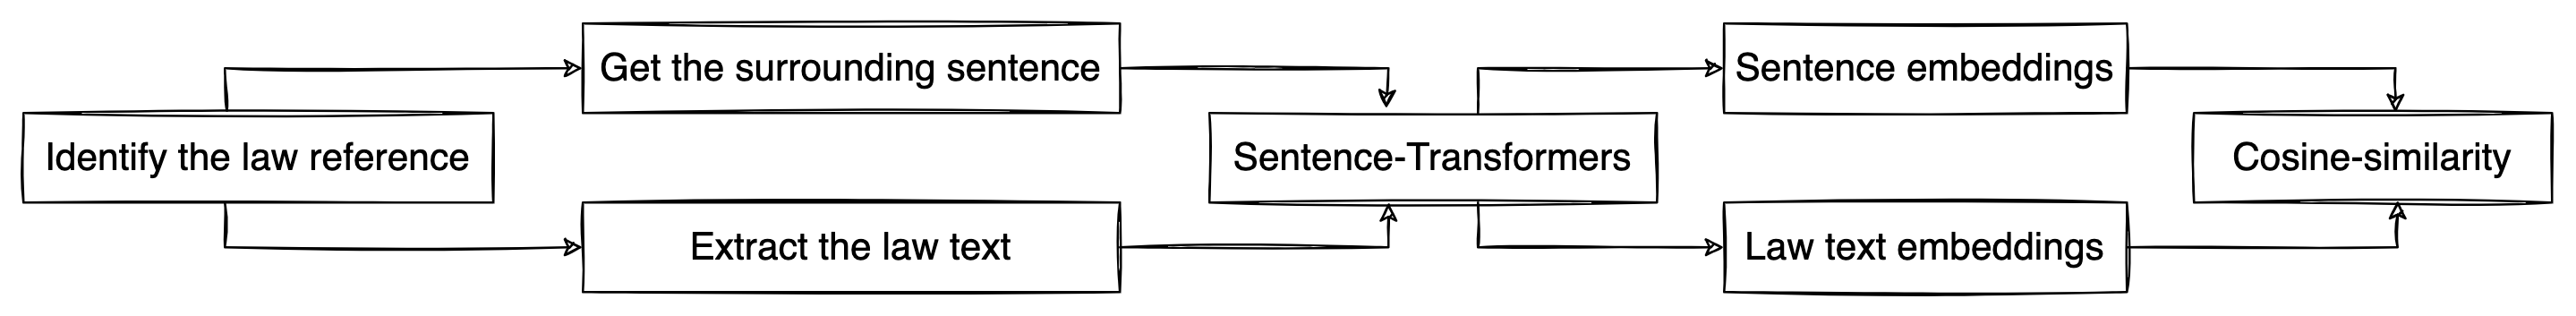
\includegraphics[width=1.0\linewidth]{images/paper_experiment.png}
	\caption{Diagram depicting the simplified process of our experiment.}
	\label{fig:experiment}
\end{figure}

\subsection{Semantic similarity between legal sentences}
Next, we use the same embedding of legal sentences and plot a t-SNE visualization in 2-dimension. However, instead of checking for legal sentences that refer to the exact Absatz in a law reference, we only look for the semantic similarity based on the base law referred. For example, if two legal sentences refer to \textit{§ 60 Abs. 7} and \textit{§ 60 Abs. 9} respectively, we only look for the semantic similarity based on the base law referred, which is \textit{§ 60}. Considering the higher number of law references in our dataset, we only plot the embeddings of legal sentences that refer to the same law more often (figure \ref{fig:sent_per_law}).

\begin{figure}
    \centering
    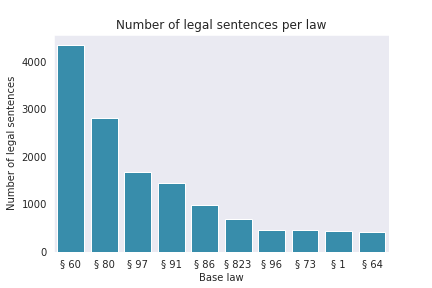
\includegraphics[width=0.8\linewidth]{images/sent_per_law.png}
    \caption{The number of legal sentences that refer to the same law.}
    \label{fig:sent_per_law}
\end{figure} 

% -------------------------------------------------------
% ----------------------- RESULTS -----------------------
% -------------------------------------------------------

\section{Results}
\label{sec:results}

Finding semantic similarities between law text and the sentences or paragraphs that refer to them is an important step towards generating or improving language models that can predict law references given legal text. In our work, we used two separate sentence transformers. In this section, we briefly compare the performance of both and the outcome of our experiment.

Embeddings generated using Cross English \& German RoBERTa for Sentence Embeddings sentence transformers achieved a median value of approximately 0.45. The highest score for this model is 0.87, and the lowest score is -0.05. A higher number of law-text and legal sentence pairs resides between a semantic similarity score of 0.35 to 0.55.

Embeddings generated using all-MiniLM-L6-v2 sentence transformers achieved a median value of approximately 0.4. The highest score for this model is 0.9, and the lowest score is -0.01. A higher number of law-text and legal sentence pairs resides between a semantic similarity score of 0.3 to 0.45.

\begin{figure}[h]
	\centering
	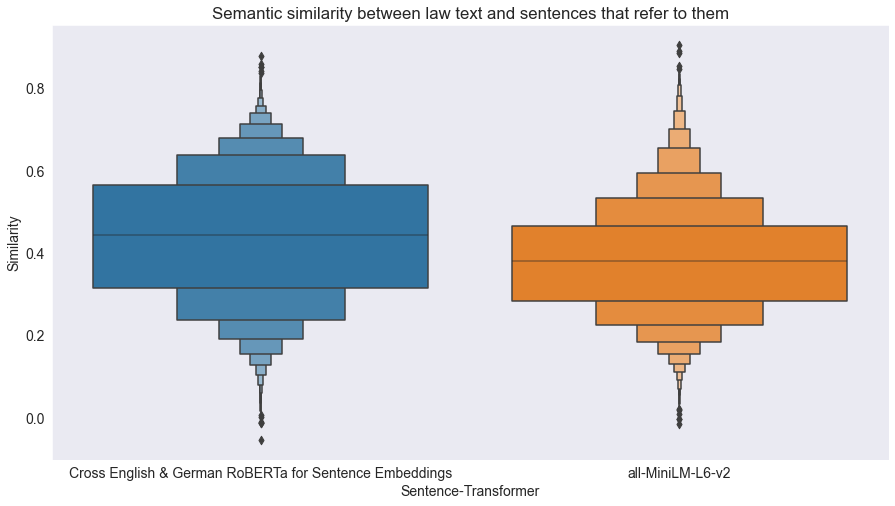
\includegraphics[width=0.9\linewidth]{images/box_sim.png}
	\caption{Box plot comparing the performance of Cross English \& German RoBERTa and all-MiniLM-L6-v2 sentence transformers. As can be seen here, the prior has higher performance than the later.}
	\label{fig:box_sim}
\end{figure}

For the same pair where Cross English \& German RoBERTa achieved the highest score, all-MiniLM-L6-v2 returns 0.84. And for the pair that later archives a high score, the former achieves 0.81. Figure \ref{fig:top-25-law-ref} shows the top-25 law references with the highest average semantic similarities.

\begin{figure}[!h]
     \centering
     \begin{subfigure}[b]{0.49\textwidth}
         \centering
         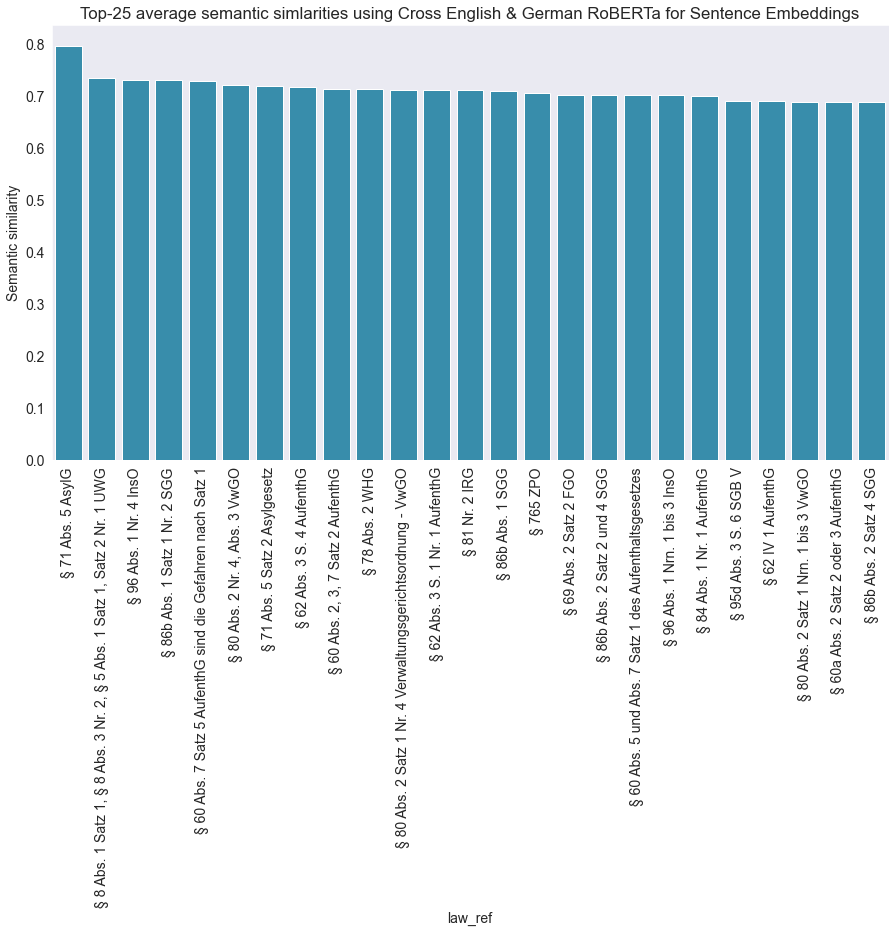
\includegraphics[width=\textwidth]{images/ts_law_sim.png}
         \caption{Cross English \& German RoBERTa for Sentence Embeddings}
     \end{subfigure}
     \hfill
     \begin{subfigure}[b]{0.49\textwidth}
         \centering
         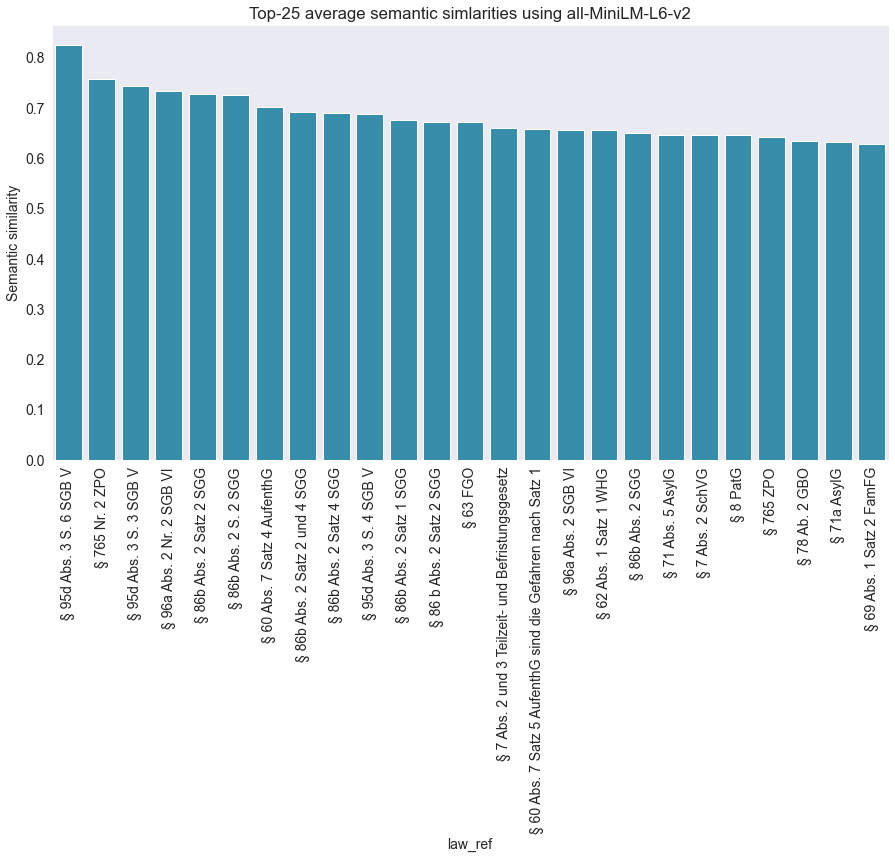
\includegraphics[width=\textwidth]{images/ml_law_sim.png}
         \caption{all-MiniLM-L6-v2}
     \end{subfigure}
    \caption{Bar chart depicting top-25 law references from our dataset that has highest semantic similarity with their surrounding text.}
    \label{fig:top-25-law-ref}
\end{figure}

We also identified the semantic similarities between legal sentences that refer to the same law. However, as mentioned in section 2, we only plot the t-SNE visualizations of embeddings of laws that have higher references in our dataset. As shown in figures \ref{fig:ts_embeddings} and \ref{fig:ml_embeddings}, it can safely be said that sentences that refer to the same law are more semantically similar and grouped together.

\begin{figure}[!h]
	\centering
	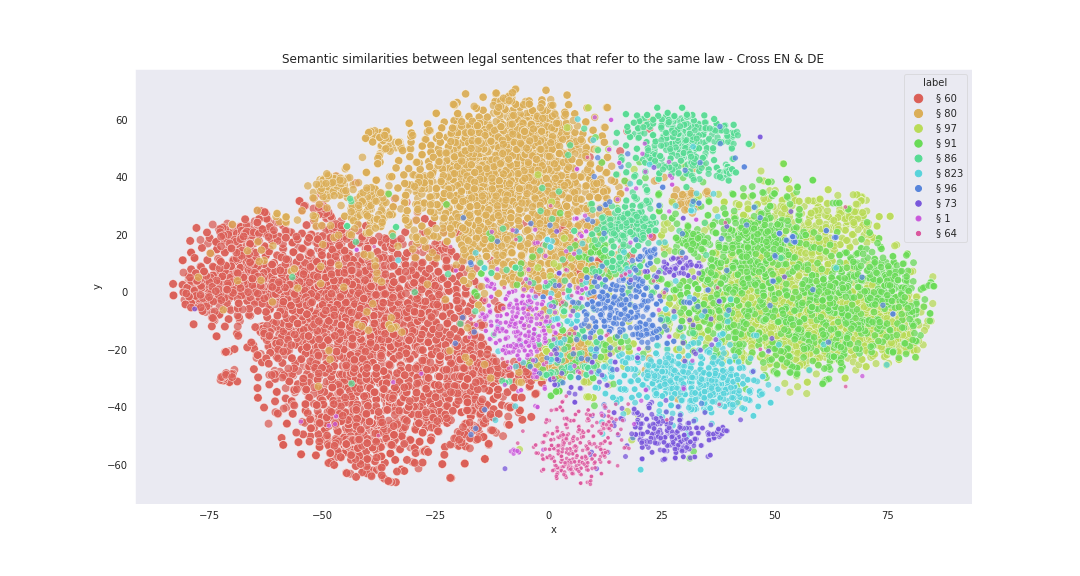
\includegraphics[width=1.0\linewidth]{images/ts_embeddings.png}
	\caption{t-SNE visualization for legal sentence embeddings achieved using Cross English \& German RoBERTa for Sentence Embeddings sentence transformer}
	\label{fig:ts_embeddings}
\end{figure}

\begin{figure}[!h]
	\centering
	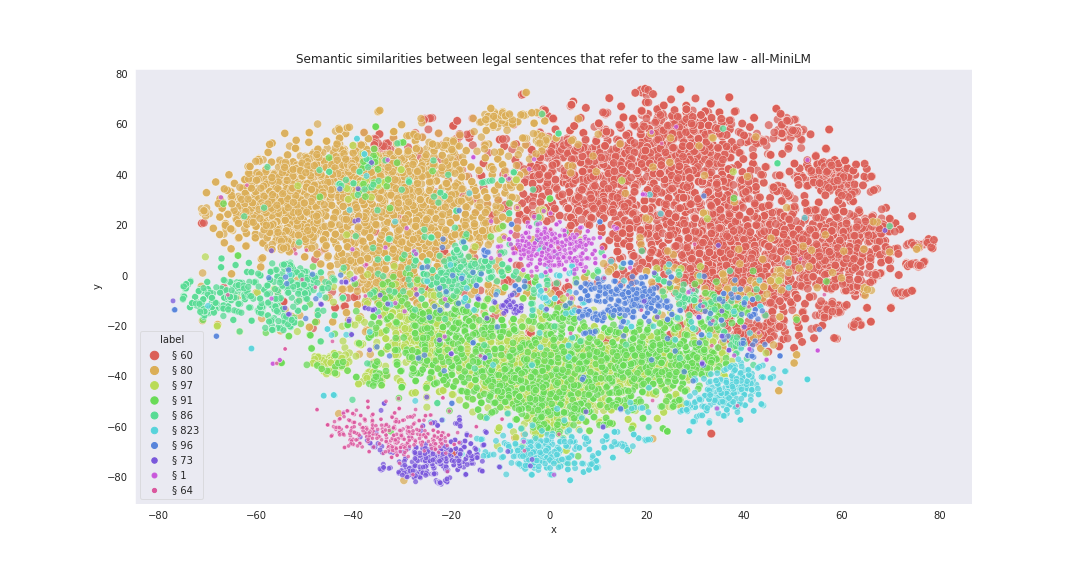
\includegraphics[width=1.0\linewidth]{images/ml_embeddings.png}
	\caption{t-SNE visualization for legal sentence embeddings achieved using all-MiniLM-L6-v2 sentence transformer}
	\label{fig:ml_embeddings}
\end{figure}

From these visualizations, it is also clear that sentence embeddings retrieved from Cross English \& German RoBERTa for Sentence Embeddings are better than all-MiniLM-L6-v2 as embeddings from prior have shown better grouping and thus higher similarity compared to the embeddings from the later. 

% -------------------------------------------------------
% --------------------- CONCLUSION ----------------------
% -------------------------------------------------------

\section{Conclusion and Future work}
\label{sec:conclusion}

In this publication, we extended the work of Milz et al. \cite{milz2021analysis} from finding similarities between court decisions to finding semantic similarities between law text and legal sentences that refer to them. We used two separate sentence transformers for our purpose. Using the embeddings from these sentence transformers, we calculate the cosine similarity between those.

In our experiment, Cross English \& German RoBERTa for Sentence Embeddings achieved slightly better performance than all-MiniLM-L6-v2. Both sentence transformers achieve a 0.45 and 0.4 similarity scores. These results show that there do exist semantic similarities between the legal text and the law text. With improved embedding techniques, this can be exploited in certain downstream tasks such as predicting law references, identifying similar court cases and court decisions, and legal text entailment.

Finally, we show that legal sentences that have the same base law reference also have a higher semantic similarity. Their embeddings in embedding space are closely grouped. We can also use this technique to distinguish between text from tenor or gründe. This will be useful when extracting text from an improperly structured dataset.

The data from the published dataset can also be used to fine-tune existing language models for various legal tasks, such as assigning NERs or predicting the case outcome.

% -------------------------------------------------------
% -------------------- BIBLIOGRAPHY ---------------------
% -------------------------------------------------------

\section{Acknowledgements}

\begin{figure}[!h]
    
\includegraphics[width=0.45\linewidth]{images/BMBF.jpg}
\end{figure}
The project on which this report is based was funded by the German Federal Ministry of Education and Research (BMBF) under the funding code 01|S20049. The author is responsible for the content of this publication.\\

\bibliographystyle{splncs04}
\bibliography{bibliography}
\end{document}
